\documentclass[12pt]{article}

% Paquetes para formato APA, márgenes y espaciado
\usepackage[main=spanish, provide=*]{babel}
\usepackage{setspace}
\usepackage[margin=1in]{geometry}
\usepackage{graphicx}
\usepackage{booktabs}
\usepackage{float}
\usepackage{amsmath}
\usepackage{caption}
\usepackage{fontspec} % Para usar fuentes del sistema
\usepackage{parskip}  % Espacio entre párrafos en vez de sangría
\usepackage{fancyhdr}
\usepackage{lipsum}   % Para texto de ejemplo
\usepackage{hyperref}
\usepackage{etoolbox}


% h


\usepackage{booktabs} % Asegúrate de cargarlo en el preámbulo



\renewcommand{\thesection}{}
\makeatletter
\renewcommand{\@seccntformat}[1]{} % Quita el número y el punto que lo sigue
\makeatother

% Fuente Calibri
\setmainfont{Carlito}

% Espaciado 1.5
% \onehalfspacing
\doublespacing


% Cabecera (si se desea)

% Portada estilo APA
\begin{document}

\begin{titlepage}
    \centering
    \vspace*{0.cm}
    \textbf{\Large Tarea 3: Modelación Logística del Crecimiento Poblacional de Estados Unidos de 1790 a 2020}\\
    \vspace{2cm}
    \begin{figure}[ht]
    \centering
    
\includegraphics[width=0.3\textwidth]{cat.jpg}
    \end{figure}

    \vspace{1.5cm}

    Ana Ximena Bravo Colín - 176820

    
    Celeste Nuñez Lopez - 176837


    Heriberto Espino Montelongo - 175199\\[2cm]

    cada cuanto es on save?

    Universidad de las Américas Puebla

    
    P25 LAT3072 1: Demografía

    Dr. Miguel Reyes 
    
    16 de mayo de 2025
\end{titlepage}

% Indice con numeración romana en mayusculas
\renewcommand{\contentsname}{Índice}
\renewcommand{\thepage}{\Roman{page}}
\pagenumbering{roman}
\setcounter{page}{1}
\tableofcontents
\newpage

% Restablecer numeración de páginas
\renewcommand{\thepage}{\arabic{page}}
\pagenumbering{arabic}
\setcounter{page}{1}

\section{Introducción}


Es un ejemplo de introducción. En este trabajo, se analiza el modelo logístico de Pearl y Reed (1920) para el crecimiento poblacional de Estados Unidos entre 1790 y 2020. El objetivo es evaluar la validez del modelo logístico en la proyección del crecimiento poblacional a largo plazo, considerando los cambios demográficos y socioeconómicos que han ocurrido desde su formulación. Para ello, se siguen los siguientes pasos:


\begin{enumerate}
\item Recopilar los datos del censo decenal de Estados Unidos (1790–1910).
\item Estimar los parámetros $a$ y $b$ del modelo logístico, suponiendo una capacidad de carga $K = 197.27$ millones.
\item Realizar interpolaciones para el periodo 1790–1910 y extrapolaciones hasta 2020.
\item Evaluar la bondad de ajuste y analizar las limitaciones del modelo.
\end{enumerate}


Pearl y Reed estimaron una capacidad de carga de aproximadamente 197 millones de personas para Estados Unidos, a partir de un ajuste empírico de la ecuación logística sobre una serie de datos censales. Este valor de $K$ representaba, bajo las condiciones tecnológicas y sociales de la época, el punto de estabilización de la población. Además del ajuste cuantitativo, los autores ofrecieron una justificación cualitativa basada en la disponibilidad de recursos: argumentaron que la tecnología y productividad agrícola vigentes imponían un límite natural a la cantidad de personas que podían ser sostenidas por la nación, dadas las restricciones en alimentos, energía y bienes esenciales.
Sin embargo, este modelo presenta limitaciones significativas al extrapolarse más allá de 1950. La capacidad de carga $K$ se basa en supuestos que no se sostienen a largo plazo, ya que la tecnología y la productividad agrícola han evolucionado drásticamente desde entonces. Por ejemplo, la Revolución Verde, los avances en energía y la globalización han transformado las dinámicas poblacionales y económicas de manera que el modelo logístico original ya no es aplicable.

Se presentan tablas comparativas, métricas de ajuste cuantitativas y una discusión crítica sobre hasta qué punto fue razonable utilizar este modelo para proyectar el crecimiento poblacional. Asimismo, examinamos las causas por las que su aplicabilidad comenzó a perder validez hacia mediados del siglo XX.



\section{Datos Censales}  % 2.1
Para reproducir el análisis original, se extrajeron las poblaciones
censales en años terminados en 0 desde la web oficial del U.S.\ Census Bureau. (U.S. Census Bureau, 2020)
Los valores se disponen en el Cuadro~\ref{tab:datos}.

\begin{table}[ht]
  \centering
  \textbf{Población de E.E.U.U.}\\
  \vspace{0.4cm}
  \begin{tabular}{cc}
    \toprule
    Año & Población real \\
    \midrule
    1790 & 3\,929\,214  \\
    1800 & 5\,308\,483  \\
    1810 & 7\,239\,881  \\
    1820 & 9\,638\,453  \\
    1830 & 12\,866\,020 \\
    1840 & 17\,069\,453 \\
    1850 & 23\,191\,876 \\
    1860 & 31\,443\,321 \\
    1870 & 38\,558\,371 \\
    1880 & 50\,189\,209 \\
    1890 & 62\,979\,766 \\
    1900 & 76\,212\,168 \\
    1910 & 92\,228\,496 \\
    \bottomrule
  \end{tabular}
    \caption{\textit{Elaboración propia}. Población de E.E.U.U. [1790--1910]}
    \label{tab:datos}
\end{table}

\newpage
\section{Estimación de Parámetros del Modelo Logístico}  % 2.2
El modelo logístico se expresa como
\[
  P(t) \;=\;
  \frac{K}{1 + \exp\bigl(a + b\,t\bigr)},
\]
donde:
\begin{itemize}
  \item $K = 197.27$M habitantes que es el límite superior al que la población se aproxima propuesta por Pearl y Reed con base en algunos supuestos cálculos en cuanto a recursos energéticos y alimenticos.
  \item $t$ = año empezando desde 1790, e.g.\ $t=0$ para 1790 y $t=10$ para 1800.
\end{itemize}
Despejando se obtiene un modelo lineal $a + b\,t$
\[
  a + b\,t \;=\;
  \textit{ln}\!\biggl(\frac{K}{P(t)} - 1\biggr)
  \;=\; T\bigl(P(t),K\bigr),
\]
Mediante regresión lineal simple se estimaron:
\[
  \hat a = 3.8960,\qquad \hat b = -0.0314.
\]
Valores que serán utilizados para la predicción de la población en el modelo logístico.

\newpage
\section{Interpolación y Extrapolación (1790--1990)}  % 2.3



 A partir de los parámetros estimados, se realizaron interpolaciones para los años $\widehat P(t)$ en el intervalo $1790\le t\le 1910$, y posteriormente se realizaron extrapolaciones para $\widehat P(t)$ en el rango $1910\le t\le 2020$. Los resultados obtenidos se presentan en el Cuadro \ref{tab:2}, junto con sus errores relativos. Al analizar estos errores, se observa que durante el siglo XIX el modelo presenta una alta precisión, con errores porcentuales mínimos que indican una estimación adecuada del crecimiento poblacional. Sin embargo, a partir de la segunda mitad del siglo XX, el error se vuelve negativo y creciente.



\begin{table}[ht]
  \centering
  \textbf{Población Real vs.\ Modelo Logístico}\\
  \vspace{0.4cm}
  \begin{tabular}{cccc}
    \toprule
    Año & Población Real & Población Modelada & Error (\%) \\
    \midrule
    1790 & 3 929 214   & 3 929 214   &          \\
    1800 & 5 308 483   & 5 339 007   &  0.005750 \\
    1810 & 7 239 881   & 7 235 700   & -0.000577 \\
    1820 & 9 638 453   & 9 771 892   &  0.013844 \\
    1830 &12 866 020   &13 135 599   &  0.020953 \\
    1840 &17 069 453   &17 548 800   &  0.028082 \\
    1850 &23 191 876   &23 257 440   &  0.002827 \\
    1860 &31 443 321   &30 507 872   & -0.029750 \\
    1870 &38 558 371   &39 505 456   &  0.024562 \\
    1880 &50 189 209   &50 355 380   &  0.003311 \\
    1890 &62 979 766   &62 995 309   &  0.000247 \\
    1900 &76 212 168   &77 142 063   &  0.012201 \\
    1910 &92 228 496   &92 282 348   &  0.000584 \\
    1920 &106 021 537  &107 729 328  &  0.016108 \\
    1930 &123 202 624  &122 739 123  & -0.003762 \\
    1940 &132 164 569  &136 648 672  &  0.033928 \\
    1950 &151 325 798  &148 983 559  & -0.015478 \\
    1960 &179 323 175  &159 502 295  & -0.110532 \\
    1970 &203 302 031  &168 177 081  & -0.172772 \\
    1980 &226 545 805  &175 135 873  & -0.226930 \\
    1990 &248 709 873  &180 595 211  & -0.273872 \\
    2000 &281 421 906  &184 803 861  & -0.343321 \\
    2010 &308 745 538  &188 004 762  & -0.391069 \\
    2020 &331 449 281  &190 414 265  & -0.425510 \\
    \bottomrule
  \end{tabular}
  \caption{\textit{Elaboración propia}. Población Observada vs.\ Predicha y Error Porcentual Individual}
  \label{tab:2}
\end{table}


Para evaluar el ajuste del modelo logístico a los datos censales, se calcularon métricas de bondad de ajuste, como el Error Absoluto Medio ($MAE$), la Raíz del Error Cuadrático Medio ($RMSE$) y el Coeficiente de Determinación ($R^2$). Los resultados de estas métricas se presentan en el Cuadro \ref{tab:metricas_logistica}, donde notamos que el modelo logístico de Pearl y Reed muestra un alto grado de precisión al interpolar la población de Estados Unidos en el periodo de 1790 a 1910, con un coeficiente de determinación $R^2$ cercano a 1 y errores bajos $MAE$ y $RMSE$, lo que indica un ajuste casi perfecto a los datos históricos. Sin embargo, al extender el modelo para realizar predicciones a largo plazo (1790–2020), el error absoluto medio $MAE$ y el error cuadrático medio $RMSE$ aumentan significativamente, reflejando una disminución en la precisión debido a cambios demográficos no capturados por el modelo. En cuanto a la extrapolación para el periodo de 1920 a 1950, los resultados muestran variación en el rendimiento, siendo el ajuste más preciso en la primera estimación que en la segunda, donde el coeficiente $R^2$ desciende considerablemente.

\begin{table}[h]
\centering
\textbf{Métricas de Bondad de Ajuste}\\
\vspace{0.4cm}
\begin{tabular}{lccc}
\toprule
\textbf{Periodo} & $MAE$ & $RMSE$ & \textbf{$R^2$} \\
\midrule
Interpolación [1790--1910] & $3.10 \times 10^5$ & $4.80 \times 10^5$ & $0.99997$ \\

Predicción total [1790--2020] & $227 \times 10^5$ & $6.92 \times 10^7$ & $0.79179$ \\

Extrapolación [1920--1950] & $22.5 \times 10^5$ & $2.68 \times 10^6$ & $0.98515$ \\

Extrapolación [1920--1950] & $761 \times 10^5$ & $8.68 \times 10^7$ & $0.66500$ \\
\bottomrule
\end{tabular}
\caption{Métricas de desempeño del modelo logístico de Pearl y Reed}
\label{tab:metricas_logistica}
\end{table}

\newpage
La Figura \ref{fig:ajuste} muestra la evolución de la población real comparada con los valores predichos por el modelo logístico. Durante el siglo XIX y hasta 1940, el modelo reproduce adecuadamente el aumento demográfico, pero a partir de 1950, comienza a estabilizarse cerca de los 200 millones de habitantes, mientras que la población real sigue creciendo. Esto sugiere que el modelo no logró captar factores contemporáneos como la inmigración o los avances en salud pública.


\begin{figure}[ht]
  \centering
  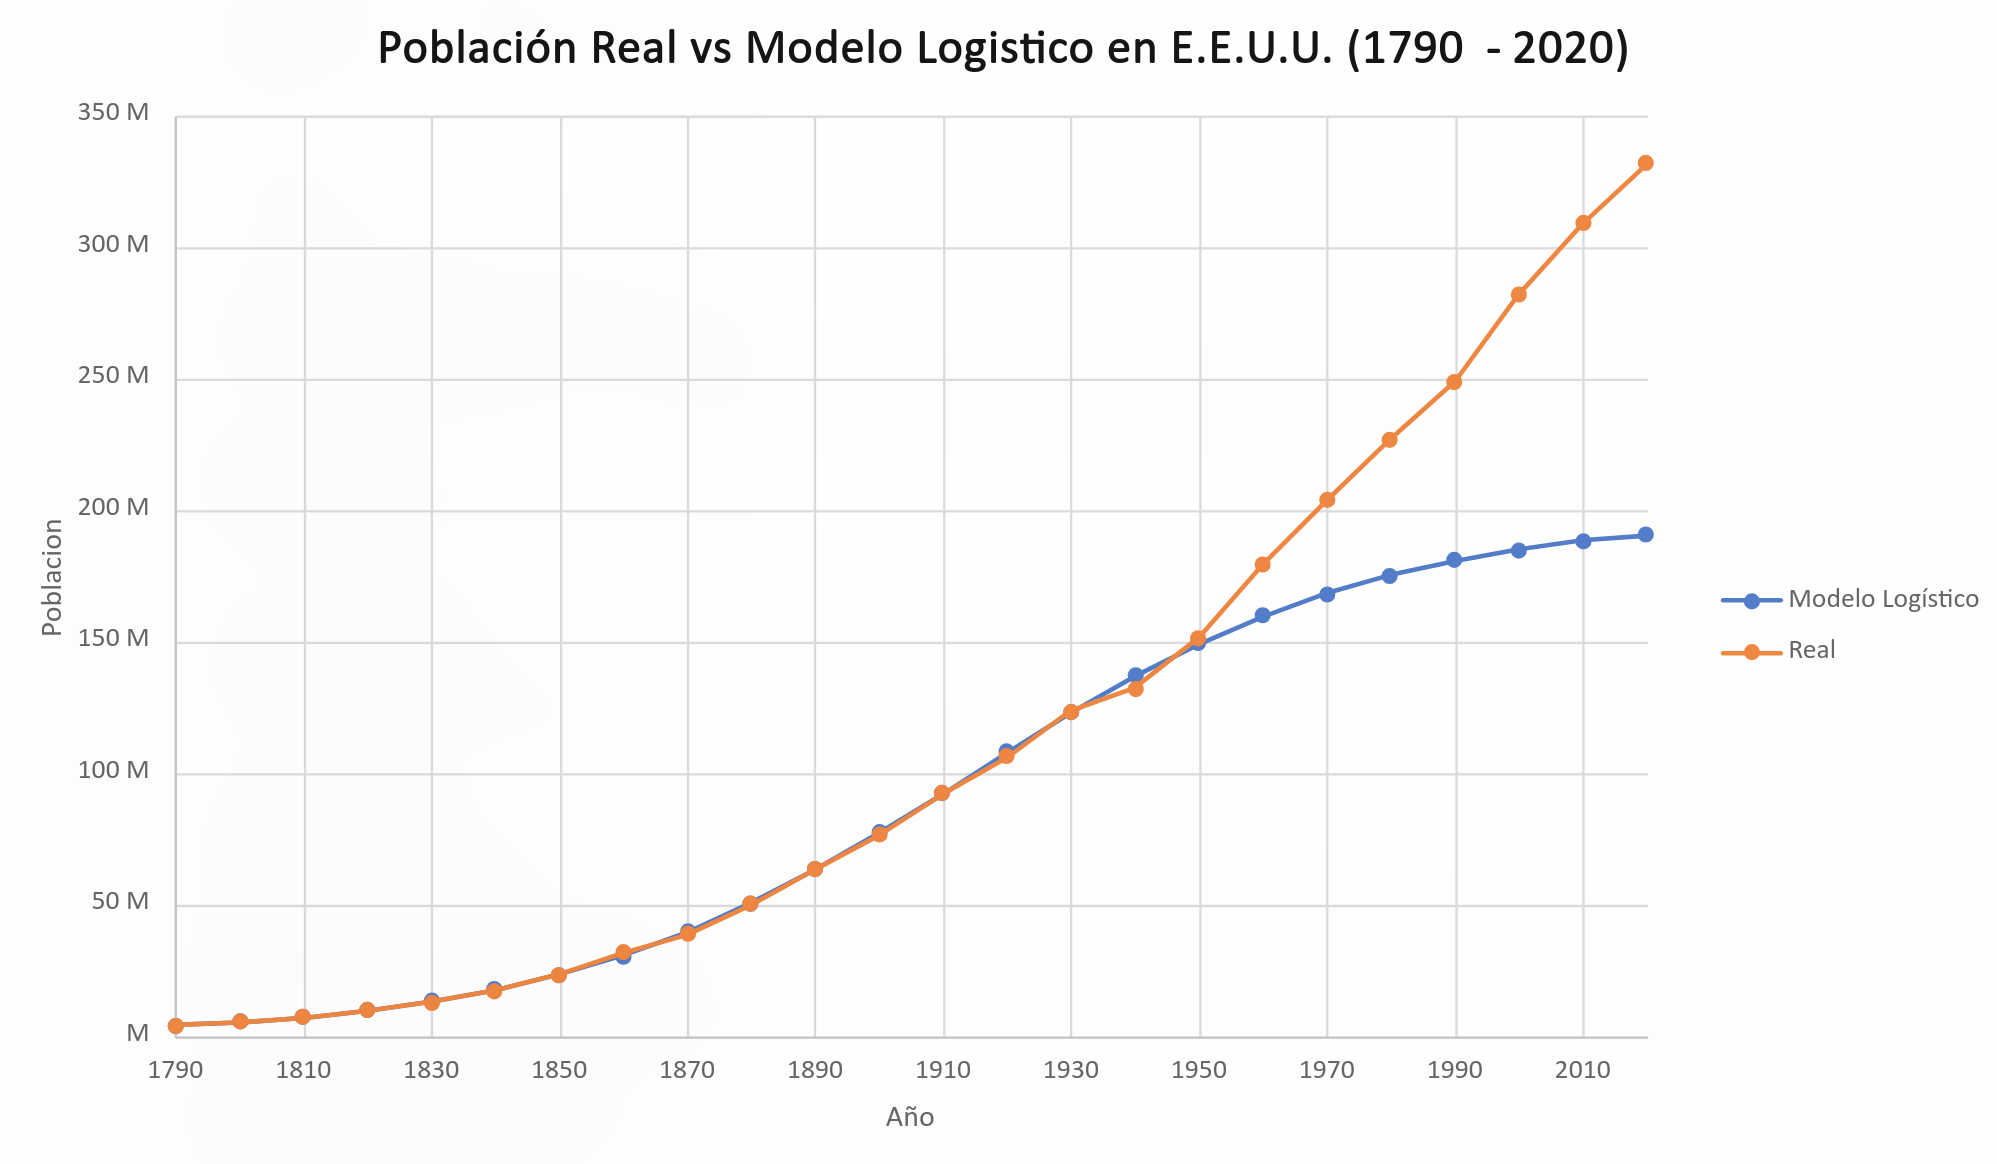
\includegraphics[width=1\textwidth]{Comparacion3.png}
  \caption{\textit{Elaboración propia}. Población real vs.\ modelo logístico [1790--1990].}
  \label{fig:ajuste}
\end{figure}

\newpage
Por último, la Figura \ref{fig:ajuste2} muestra el error porcentual individual calculado como 
$$
\text{Error} = \frac{\text{Población real} - \text{Población modelada}}{\text{Población real}} \times 100$$

Inicialmente, el error se mantiene bajo, indicando un buen ajuste, y en caso de error, estos son positivos, indicando que el modelo sobreestimo el crecimiento de la población, pero a partir de mediados del siglo XX, el error se incrementa drásticamente hacia valores negativos, mostrando que el modelo subestima la población en las últimas décadas.
 
\begin{figure}[ht]
  \centering
  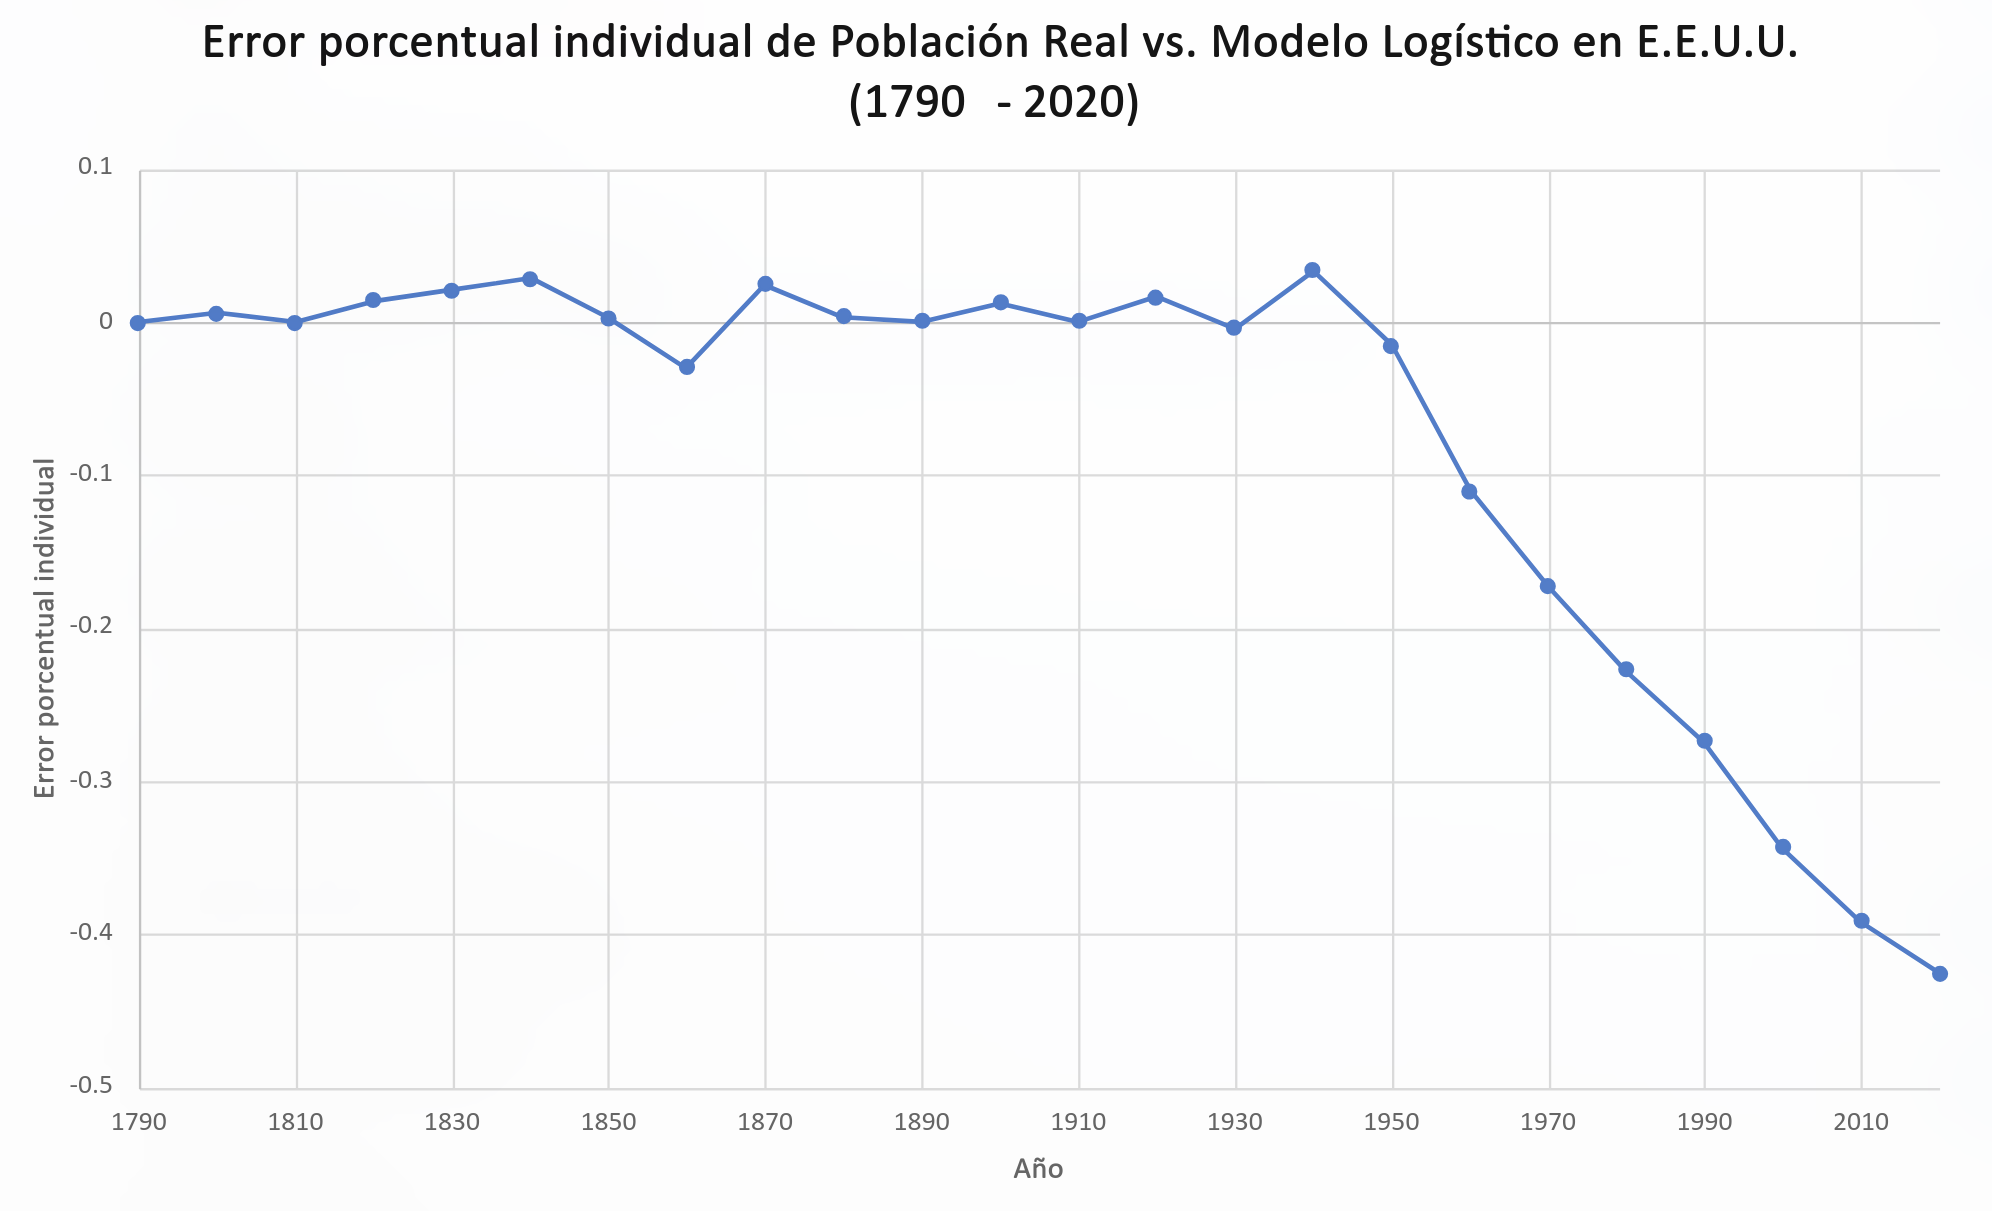
\includegraphics[width=1\textwidth]{Error3.png}
  \caption{\textit{Elaboración propia}. Errores porcentuales del modelo logístico [1790--2020].}
  \label{fig:ajuste2}
\end{figure}




\newpage
\section{Conclusión}

El modelo logístico de Pearl y Reed fue altamente efectivo para modelar el crecimiento poblacional de Estados Unidos durante el periodo de 1790 a 1910, ya que capturó con precisión las tres fases clásicas del crecimiento: una etapa inicial de crecimiento lento, seguida de una fase de aceleración exponencial y finalmente una ralentización coherente con las limitaciones energéticas y alimenticias de la época (Pearl \& Reed, 1920). Como se mencionó anteriormente, para este periodo el coeficiente de determinación ($R^2$) cercano a 1 y un error cuadrático medio ($RMSE$) bajo con errores porcentuales mínimos, lo que indica un ajuste casi perfecto con una estimación adecuada. El límite superior al que la población se aproxima de $K = 197.27$ millones resultaba razonable bajo las condiciones tecnológicas y socioeconómicas vigentes a principios del siglo XX (Smith \& Keyfitz, 1977). Por lo tanto, hasta aproximadamente el año 1950, el modelo logístico seguía siendo una herramienta útil y precisa para proyectar el crecimiento poblacional, manteniendo errores porcentuales por debajo del 4\% (Preston et al., 2001).

Sin embargo, notamos que a partir de la década de 1950, el modelo comenzó a perder precisión, reflejándose en errores negativos y crecientes. Esto se debe a que el modelo no contempló cambios estructurales que modificaron drásticamente la relación entre población y recursos. Entre los factores que influyeron destacan la Revolución Verde, que aumentó la productividad agrícola mediante técnicas innovadoras (Pingali, 2012); la expansión energética, con el uso masivo de petróleo, gas y electricidad (Smil, 2003); los cambios demográficos impulsados por grandes flujos migratorios (Hirschman, 2005); los avances sanitarios que redujeron la mortalidad y aumentaron la esperanza de vida (Cutler et al., 2006); y, de forma crítica, las transformaciones socioeconómicas y demográficas derivadas de la Segunda Guerra Mundial y el baby boom posterior (Jones, 2003).

La Segunda Guerra Mundial marcó un punto de inflexión, ya que impulsó una movilización industrial sin precedentes, consolidó el liderazgo tecnológico de Estados Unidos y fomentó la urbanización (Galbraith, 1958). Asimismo, la apertura migratoria con la Ley de Inmigración de 1965 contribuyó al crecimiento poblacional acelerado (Massey et al., 1993). Estas transformaciones estructurales modificaron la relación entre el consumo de energía y los recursos disponibles por persona, lo que provocó que el límite superior al que la población se aproxima inicialmente calculado quedará desfasado, haciendo que el modelo logístico perdiera validez para proyecciones después de 1950.

En conclusión, aunque el modelo logístico fue una herramienta útil para analizar el crecimiento poblacional durante el siglo XIX y principios del XX, su extrapolación a largo plazo resultó limitada debido a la incapacidad de prever cambios significativos en la dinámica demográfica y socioeconómica. Esto remarca la importancia de contar con modelos más flexibles que puedan adaptarse a contextos históricos cambiantes y que incorporen variaciones en el límite superior al que la población se aproxima provocadas por innovaciones tecnológicas y políticas migratorias.


\newpage
\begin{thebibliography}{99}

\bibitem{cohen1995}
Cohen, J. E. (1995). \textit{How many people can the Earth support?} W. W. Norton \& Company.

\bibitem{cutler2006}
Cutler, D. M., Deaton, A. S., \& Lleras-Muney, A. (2006). The determinants of mortality. \textit{Journal of Economic Perspectives}, \textit{20}(3), 97--120. \url{https://doi.org/10.1257/jep.20.3.97}

\bibitem{galbraith1958}
Galbraith, J. K. (1958). \textit{The affluent society}. Houghton Mifflin.

\bibitem{hirschman2005}
Hirschman, C. (2005). Immigration and the American century. \textit{Demography}, \textit{42}(4), 595--620. \url{https://doi.org/10.1353/dem.2005.0031}

\bibitem{jones2003}
Jones, L. (2003). \textit{Great expectations: America and the Baby Boom generation}. Basic Books.

\bibitem{massey1993}
Massey, D. S., Durand, J., \& Malone, N. J. (1993). \textit{Beyond smoke and mirrors: Mexican immigration in an era of economic integration}. Russell Sage Foundation.

\bibitem{pearl1920}
Pearl, R., \& Reed, L. J. (1920). On the rate of growth of the population of the United States since 1790 and its mathematical representation. \textit{Proceedings of the National Academy of Sciences}, \textit{6}(6), 275--288. \url{https://doi.org/10.1073/pnas.6.6.275}

\bibitem{pingali2012}
Pingali, P. L. (2012). Green revolution: Impacts, limits, and the path ahead. \textit{Proceedings of the National Academy of Sciences}, \textit{109}(31), 12302--12308. \url{https://doi.org/10.1073/pnas.0912953109}

\bibitem{smil2003}
Smil, V. (2003). \textit{Energy at the crossroads: Global perspectives and uncertainties}. MIT Press.

\bibitem{smith1977}
Smith, D. P., \& Keyfitz, N. (1977). \textit{Mathematical demography: Selected papers}. Springer.

\bibitem{census2020}
U.S. Census Bureau. (2020). \textit{Decennial census by decade}. \url{https://www.census.gov/programs-surveys/decennial-census/decade.html}

\end{thebibliography}




\end{document}
